\documentclass[thesis.tex]{subfiles}
\begin{document}
\chapter{Recasting Text Simplification as a Document Retrieval Task}
\label{chap:retrieval}

In the previous chapters, we have discussed the state of current lexical and sentence-level simplification systems and proposed ways to extend and improve upon them. While these approaches have proven to be useful in downstream natural language processing tasks, they still have several crucial limitations that prevent these models from being practically useful. First, the models still make many fluency and adequacy errors. These errors are particularly pronounced when models are presented with very long and complex sentences, which makes it difficult to scale up these methods in order to simplify entire documents. In addition, while these models view complexity as a binary Complex to Simple English translation task, complexity is not a binary notion; what is considered complex for one person or group of people may be quite simple for another.

Apart from these issues, when we consider learners who wish to acquire knowledge about a new topic or skill, it is clear that they generally need to understand the totality of a text about this topic. However, often times there are many phrases in a text that cannot be more easily understood just by replacing them with simpler substitutes. As an example, let's consider this excerpt from Wikipedia on \textit{Machine Learning}: \\

\noindent\fbox{%
    \parbox{\textwidth}{%
        Machine learning (ML) is the scientific study of \textbf{\textit{algorithms}} and \textbf{\textit{statistical models}} that computer systems use to carry out tasks without explicit instructions....Machine learning algorithms build a mathematical model based on \textbf{\textit{sample data}}, known as training data, in order to make predictions or decisions without being explicitly programmed to do so.
    }%
} \\\\

In order to understand this passage, a reader needs to have prior knowledge of the meaning of phrases such as \textit{algorithms}, \textit{statistical models}, and \textit{sample data}. If the reader does not know what these phrases (or \textbf{\textit{Concepts}}) mean, they will need to be provided with an explanation. In some cases, it may be enough to provide a definition describing this, as with \textit{sample data} in the above example. However, for many phrases corresponding to relatively complex concepts, such as \textit{algorithms}, it is likely necessary to read longer descriptions written at an appropriate level for the learner.

Due to these issues, rather than focusing on continuing to improve current simplification models, we propose to instead reformulate the problem of text simplification, setting as our goal to help a user learn about a topic with which they may not be familiar. To make the task more tractable, if we start with a document $D$ on a given topic, we can break down the task into three sub-tasks. The first is \textbf{Concept Identification}, where we need to identify the concepts within $D$ that are critical for understanding that document. The second task is \textbf{Leveled Document Retrieval}, where for each concept $c$, we need to retrieve a set of documents $D^{\prime}$ related to $c$ from a $variety$ of complexity levels, before re-ranking this set to find documents that are at levels most appropriate for the user.

\section{Critical Concept Identification} \label{sec:concept}

The first step in our proposed approach is to identify the important concepts inside a document. That is, given a document, we want to be able to extract all concepts that are critical to understanding its content. This task can be broken down into two sub-problems: \textit{candidate concept identification}, where we identify all words and multiword expressions that could potentially form a concept; and \textit{candidate score computation}, where we calculate a score for each candidate $c$ that approximates the likelihood of $c$ being a concept.

\subsection{Methods}

Early works on keyword extraction focused on formulating this as a supervised classification task, using features such as the frequency of the most common token, the relative number of characters, and the first relative occurrence of a phrase component \citep{turney2000learning}. \cite{hulth2003improved} further showed that incorporating part-of-speech features leads to further improvements in performance. In this work, as our goal is to extract concepts from texts of various domains, we choose to focus mainly on unsupervised approaches.

The first work we compare to is \cite{mihalcea2004textrank}. They reformulate the keyword extraction task as a graph-based ranking problem. Specifically, given a document $D$, they propose to produce a directed graph $G = (V, E)$, where each vertex $v \in V$ represents a single word (i.e. a potential keyword); only nouns and adjectives are considered as potential keywords. A pair of vertices ($v_1$, $v_2$) is connected by an edge $e \in E$ if the words associated with these vertices co-occur within a window of $N$ words, where $N$ is a hyperparameter to be tuned through experimentation. The score $S(v_i)$ of each vertex $v_i$ is initialized to 1, and then updated during each iteration of the algorithm as follows:

\begin{equation}
S(v_i) = (1 - d) + d*\sum_{j \in In(v_i)} \frac{1}{Out(v_j)} * S(v_j)
\end{equation}

$In(v_i)$ represents the set of vertices that have an edge pointing towards a vertex $v_i$, $Out(v_i)$ represents the set of vertices pointed to from $v_i$, and $d$ is a dampening parameter, set to 0.85 \citep{mihalcea2004textrank}. The top $t$ keywords, as ranked after the algorithm has converged, are passed through a post-processing step which combines adjacent adjectives and nouns if both are identified as keywords.

Subsequent work has attempted to leverage multi-word expressions more directly, as single words can be used in many different contexts; a notable example of this is Rapid Automatic Keyword Extraction, or RAKE \citep{rose2010automatic}. This approach generates a set of stopwords and phrase delimiters, and leverages this to partition a document into a set of candidate keywords. RAKE creates a graph of word co-occurrences $G$, meaning that two words have an edge between them when they are found in the same candidate. A score is then computed for each word $w$ based on its frequency ($freq(w)$), the degree of its corresponding vertex in $G$ ($deg(w)$), and the ratio between its degree and its frequency ($\frac{deg(w)}{freq(w)}$); finally, an overall score is computed for each candidate by taking the sum of its word scores. To account for concepts that contain stopwords (e.g. \textit{axis of evil}) candidates that are found adjacent and in the same order multiple times within a document are combined. RAKE returns the top $t$ percentage of candidates as true keywords; in this work, $t$ is set to 0.33.

Similar to RAKE, YAKE (Yet Another Keyword Extractor) is a multilingual unsupervised algorithm that uses features extracted from a single document and only requires a static list of stopwords as external data \citep{campos2020yake}. After applying a similar pre-processing step as the RAKE algorithm, YAKE computes five features for each word: \textit{casing} (i.e. the capitalization of a word); \textit{word positional} (i.e. the relative position of the word within the document); \textit{word frequency} (i.e. the frequency of a word within the document); \textit{word relatedness to context} (i.e. the number of unique word that occur close to a term); and \textit{Word DifSentence} (i.e. how often a word appears in distinct sentences). Each word $w$ is then assigned a score $S(w)$, and each keyword $k$ is assigned a score as follows (here, $TF(k)$ represents the term frequency of $k$):

\begin{equation}
S(w) = \frac{\prod_{w \in k} S(w)}{TF(k) * (1 + \sum_{w \in k} S(w))}
\end{equation}

Note that unlike RAKE, there is an extra normalization step, which serves to avoid artificially inflating the scores of longer $n$-grams. Finally, YAKE outputs a list of keywords sorted by the score, where a lower score indicates a more important phrase.

In our work, we also consider several methods that extend previous approaches. In order to create our own method, we first need to extract all candidate concepts from a document. This is a non-trivial task, as there is potentially an exponential number of possible phrases that can be extracted from a single document. Previous methods often focus on $n$-gram-based  approaches for candidate identification, which allow the models to be relatively quick and scalable; however, these can result in poor phrasal boundaries, sometimes mixing verbs and nouns in the same phrase. In this work, what we only consider noun phrases ``candidate concepts". We thus choose to use the candidates identified by YAKE for all of our extended methods, as true candidates must be contained within a single chunk within a sentence.

Several recent works have naturally leveraged Wikipedia for concept identification and entity linking \citep{ratinov2011local,upadhyay2018joint}, as it contains a millions of articles about specific topics or entities. To organize these documents, Wikipedia labels each document with a set of categories. These categories are also organized into a sort of hierarchy; for example, the subcategories under ``Computer Science" include ``Artificial Intelligence" and ``Computer Architecture". This allows us to extract a large set of concepts relevant to a target domain. Most of our proposed methods leverage these categories. One issue with extracting concepts this way is that this ``hierarchy" actually contains many cycles, i.e. following this hierarchy all the way to the bottom results in many irrelevant categories. For example, attempting to build a complete hierarchy of concepts starting under ``Computer Science" eventually results in the inclusion of categories such as ``flower", which is clearly an out-of-domain concept. This is an issue we need to keep in mind as we use this large-scale general corpus. To get around this, we extracted a hierarchy of concepts that were at most eight steps beneath ``Computer Science", our target domain for these experiments. This process results in 106,359 categories. If we also include the titles of all Wikipedia pages labeled with these categories, this results in 792,555 total Computer Science-related concepts. We leverage these as baseline methods (\textbf{Wiki-Cat} and \textbf{Wiki-All}) by performing a simple dictionary lookup or each candidate concept.

Inspired by recent work that applies BERT-based models to keyphrase extraction \citep{sharma2019self}, we consider several unsupervised approaches leveraging pre-trained language models. In our first approach, given a document text $t$ and each candidate concept $c \in C$ identified within $t$, we generate a score for $c$ by calculating the cosine similarity between the SBERT embeddings of $t$ and $c$; we refer to this method as \textbf{DocSim}.\footnote{This can be considered a variation of KeyBERT https://github.com/MaartenGr/KeyBERT.} Note that we use SBERT over BERT here as SBERT embeddings were created to make similarity comparisons more meaningful \citep{reimers2019sentence}.

One potential issue with this first approach is that the number of words in the entire document is much larger than the number of words in a single candidate concept, thus the similarity between embeddings may not be the most meaningful. To get around this issue, we also consider comparing each candidate $c \in C$ by computing its SBERT embedding similarity to a document's title; we refer to this method as \textbf{TitleSim}.

While using the title significantly cuts down on the number of words, it is important to note that the title often contains stopwords such as ``the" and ``of" that could make this process less accurate, resulting in some relevant concepts still being excluded. Thus, we also extend the method of \cite{tsai2013concept}, which compares each candidate concept to concepts in a small manually collected seed dictionary. In our experiment, to create our seed dictionary, we take the top-$k$ most relevant concepts based on their SBERT embedding similarity to the document title; we choose $k$ = 2 through experimentation. For each candidate concept $c \in C$ we then compute the maximal embedding similarity between $c$ and the seed concepts.

\subsection{Data Collection}

For evaluation, previous work has mainly leveraged corpora consisting of abstracts from technical articles. \cite{mihalcea2004textrank} and \cite{rose2010automatic} both evaluate TextRank and RAKE, respectively, on the 500 test texts from the Inspec dataset, which consist of abstracts from journal papers in the Computer Science and Information Technology domain. Similarly, \cite{tsai2013concept} evaluate on a set of abstracts taken from the ACL Anthology annotated with concepts identified as either \textit{focus}, an article's main contribution; \textit{technique}, a method or tool used in the article; and \textit{domain}, an article's application domain \citep{gupta2011analyzing}.

In our work, while technical abstracts are helpful to consider, we also want to determine the efficacy of these models on web-based articles as well. Thus, we extract a set of 41 web-based articles from the computer science domain, and train two annotators to manually annotate concepts for each document. These articles are from the following sources:

\begin{itemize}
\setlength\itemsep{-1em}
\item Seven abstracts from the journal \textit{Data Science}.
\item Nine articles from \textit{Edureka} and \textit{Intellipaat}, two introductory computer science websites.
\item Eleven articles from \textit{python-course.eu} and  \textit{python.swaroopch.com}, websites with introductory Python articles.
\item Seven articles from \textit{GeeksforGeeks}, a website with a variety of technical and coding computer science articles and problems.
\item Five articles from \textit{Wikipedia}.
\item Two articles from \textit{marksheet.io}, a website focused on introductory HTML articles.
\end{itemize}

The guidelines given to annotators are described in Appendix \ref{app:concept_guidelines}. After the initial annotation process, the annotators were asked to perform an additional adjudication for each phrase that was disagreed upon. In order to determine the level of agreement between annotators, we compute Cohen's Kappa coefficient. The general formula for Cohen's Kappa is below; here, $p_e$ represents the expected probability of an event occurring, and $p_o$ represents the observed probability that the event occurred:

\begin{equation}
\kappa = \frac{p_o - p_e}{1 - p_e}
\end{equation}

To compute this, we can formulate our problem as follows: for each candidate concept $c \in C$, each annotator gave either a positive label (i.e. $c$ is a critical concept) or a negative label ($c$ is not a critical concept). We can compute \textit{Equal Kappa}, where we weight agreement on positive and negative labels equally. We make the assumption that the expected probability of identifying $c$ as a concept is 0.5.

\begin{equation}
p_e = P(Binary\;Agreement) = 0.5
\end{equation}
\begin{equation}
p_o = \frac{\#\;Total\;agreed\;upon\;annotations}{\#\;Total\;noun\;phrases}
\end{equation}

To compute the total number of noun phrases, we generate a full constituency parse of each sentence in each article, and extract all non-nested noun phrases.\footnote{We generate the constituency parse using Spacy's python implementation of the Berkeley Neural Parser \cite{kitaev2018constituency}.} Note that these articles are all from the computer science domain, so they often contain mathematical equations and/or coding snippets. To reduce confusion for the constituency parser (as well as any concept extraction models later on), we use html tags to automatically remove code snippets from our test articles, and manually clean the remaining.

While Equal Kappa is reasonable at first glance, the main issue with this metric is that the expected probability in our task is really not 0.5, as there are significantly more noun phrases than there are identified concepts. Thus, we propose a second agreement metric, called \textit{Positive Kappa}, where we only focus on agreement for phrases identified as concepts.

\begin{equation}
p_e = \frac{\#\;Annotator\;1\;concepts + \#\;Annotator\;2\;concepts}{2 * \#\;Total\;noun\;phrases}
\end{equation}
\begin{equation}
p_o = \frac{\#\;Total\;agreed\;upon\;concepts}{\#\;Total\;identified\;concepts}
\end{equation}

\begin{table*}
\begin{center}
\small
\begin{tabular}{|c|c|c|} \hline
& Equal Kappa & Positive Kappa \\ \hline
Pre-Adjudication & 0.806 & 0.272 \\ 
Post-Adjudication & 0.841 & 0.488 \\ \hline
\end{tabular}
\end{center}
\caption{\label{tab:kappa_agreement} Annotation agreement metrics before and after the secondary adjudication step.}
\end{table*}

To use an example, if there are 100 total noun phrases, and Annotator 1 identified 10 concepts, while Annotator 2 identified 15 concepts, the expected agreement, i.e. if these were identified at random, would be $\frac{10 + 15}{2*100}$ = 0.125. The agreement metrics before and after adjudication are shown in Table \ref{tab:kappa_agreement}. As expected, having our annotators do a second pass where they focus on cases of disagreement results in a significant increase in positive Kappa. Finally, to generate a single set of gold concepts for each document, we only use concepts that were identified by both annotators; in total, this results in 657 concepts identified in the 41 documents of our dataset.

\subsection{Experiments}

We compare different standard keyphrase extraction methods with additional baseline and BERT-based approaches. For several methods, we use different ranking thresholds to filter out different numbers of candidate concepts. For example, a ranking threshold of 1 means that we will use all the candidate concepts, effectively ignoring the model ranking; on the other hand, a ranking threshold of 0.33 means that we will take only the top 33\% candidates in the ranking produced by some method.

We compare the following methods:

\begin{itemize}
\setlength\itemsep{-1em}
\item Mapping to all computer science Wikipedia categories (\textbf{Wiki-Cat}), starting with all candidate concepts identified by YAKE \citep{campos2020yake}.
\item Mapping to all computer science Wikipedia categories and article titles (\textbf{Wiki-All}), starting with all candidate concepts identified by YAKE.
\item \textbf{TextRank} \citep{mihalcea2004textrank}, using ranking thresholds of 1 and 0.33.\footnote{We use the Python implementation of TextRank \citep{paco2016pytextrank} integrated into the SpaCy framework (www.spacy.io).}
\item \textbf{RAKE} \citep{rose2010automatic}, using ranking thresholds of 1, 0.33, and 0.2.\footnote{We use the Python implementation of RAKE at https://github.com/aneesha/RAKE.}
\item \textbf{YAKE} \citep{campos2020yake}, using ranking thresholds of 1, 0.33, 0.2, and 0.1.
\item \textbf{KeyBERT}, a simple BERT-based approach based on \cite{sharma2019self}, using ranking thresholds of 1 and 0.33.\footnote{We use the Python implementation found at https://github.com/MaartenGr/KeyBERT.}
\item \textbf{DocSim}, an SBERT-based approach comparing candidate concepts to the embedding of the entire document; starting with candidate concepts identified by YAKE, using a ranking threshold of 0.33.
\item \textbf{TitleSim}, an SBERT-based approach comparing candidate concepts to a document's title; starting with candidate concepts identified by YAKE, using a ranking threshold of 0.33.
\item \textbf{SeedSim}, an SBERT-based approach first comparing candidate concepts to a document's title, identifying $k$ seed concepts, before comparing candidates to the seed concepts; starting with candidate concepts identified by YAKE, using a ranking threshold of 0.33.
\end{itemize}

\begin{table*}
\begin{center}
\small
\begin{tabular}{|c|c|c|c|c|} \hline
\textbf{Method} & \textbf{Threshold} & \textbf{Precision} & \textbf{Recall} & \textbf{F-Score} \\ \hline
Wiki-Cat & -- & 0.200 & 0.143 & 0.167 \\
Wiki-All & -- & 0.183 & 0.311 & 0.231 \\ \hline
\multirow{2}{1.5cm}{\centering TextRank} & 1 & 0.097 & 0.469 & 0.160 \\
& 0.33 & 0.199 & 0.310 & 0.242 \\ \hline
\multirow{3}{1.5cm}{\centering RAKE} & 1.0 & 0.119 & 0.766 & 0.212 \\ 
& 0.33 & 0.168 & 0.363 & 0.230 \\ 
& 0.2 & 0.189 & 0.250 & 0.215 \\ \hline
\multirow{4}{1.5cm}{\centering YAKE} & 1.0 & 0.075 & \textbf{0.943} & 0.139 \\
& 0.33 & 0.177 & 0.401 & 0.246 \\
& 0.2 & 0.219 & 0.303 & \textbf{0.254} \\
& 0.1 & \textbf{0.268} & 0.189 & 0.221 \\ \hline
\multirow{2}{1.5cm}{\centering KeyBERT} & 1.0 & 0.027 & 0.898 & 0.053 \\
& 0.33 & 0.024 & 0.156 & 0.042 \\ \hline
TitleSim & 0.33 & 0.149 & 0.272 & 0.183 \\
SeedSim & 0.33 & 0.132 & 0.272 & 0.177 \\
DocSim & 0.33 & 0.137 & 0.175 & 0.153 \\ \hline
\end{tabular}
\end{center}
\caption{\label{tab:concept_evaluation} Comparison of concept identification methods on our manually annotated test set.}
\end{table*}

The results are shown in Table \ref{tab:concept_evaluation}. As we can see, surprisingly all models that leverage large pre-trained language models perform quite poorly on our evaluation set. Regarding KeyBERT, this is likely due to the $n$-gram-based approach to identifying candidate concepts being quite noisy. In addition, comparing candidate concept embeddings to that of the entire document likely is an inappropriate comparison, due to the sheer difference in number of words. Regarding our methods relying on the title, this seems like a reasonable approach when the title is a technical concept or a combination of concepts related to the document; however, in our dataset this seems to often not be the case. For example, one of the Wikipedia articles is entitled \textit{TenTen Corpus Family}; the title of a corpus followed by the word \textit{family} is likely not a meaningful phrase to compare to in embedding space. Looking at the results overall, YAKE slightly outperforms all other baselines, though our simple dictionary lookup using Wikipedia computer science topics is surprisingly competitive.

\section{Complexity Level-Sensitive Document Retrieval} \label{sec:retrieval}

For a given complex document, our task is to retrieve documents on the same topic but written at different complexity levels. This means that our document-level representation should be able to capture semantic similarity across levels. A challenge for this task is that the vocabulary used in a simple document is generally quite different from that used in complex documents, making it difficult to use standard TF-IDF-based retrieval methods. Therefore, we instead experiment with several different contextual embedding representations.

We leverage recent advancements in BERT-based language models \citep{devlin2019bert,reimers2019sentence}, and explore their ability to capture both semantic (topic) similarity and text complexity. As BERT-based models can process up to 512 WordPiece tokens (henceforth tokens) at a time, it is not possible to generate a single embedding for an entire document $D$ at once. Thus, we split $D$ into a set of paragraphs \textbf{P}, denoted in $D$ through new line markers, and combine them into text segments $S_i \in D$ of length up to 512 tokens. We generate embeddings for these text segments $\textbf{E}_{S_i}$ and compute their average weighted by their length ($l_{S_i}$). Formally, we compute each dimension $e_j \in \textbf{E}_D$ of our document-level embedding as follows:

\begin{equation*}
e_j = \frac{\sum_{S_i} e_{S_i, j} * l_{S_i}}{\sum_{S_i} l_{S_i}}
\end{equation*}

\noindent Given an input document $D_s$ and a set of documents $D_t$ in a corpus $\textbf{C}$, we rank the documents in $C$ based on the cosine similarity of their embeddings $E_{D_t}$ to that of the input, $E_{D_s}$.

\begin{equation*}
    sim(D_{s}, D_{t}) = cos\_sim(E_{D_s}, E_{D_t})
\end{equation*}

In this experiment, we use both BERT \citep{devlin2019bert} and Sentence-BERT (SBERT) \citep{reimers2019sentence} pre-trained embeddings. As SBERT generates sentence-level embeddings that are more semantically meaningful \citep{reimers2019sentence}, we expect that SBERT will outperform BERT. Apart from directly using static pre-trained embeddings, we also attempt a fine-tuned approach. To do so, we adapt the Siamese BERT-network architecture introduced by SBERT \citep{reimers2019sentence} with the goal of learning that texts on the same topic at different complexity levels are similar, while texts about different topics at the same complexity level are not similar. We do this by fine-tuning a Siamese BERT network on a binary classification task. The positive examples (labeled 1) consist of an aligned text pair ($T_{ij}$, $T_{ij^{\prime}}$) containing similar content, where $T_{ij^{\prime}}$ is at a lower complexity level than $T_{ij}$. The negative examples (labeled 0) consist of a non-aligned text pair (different content) written at the same complexity level ($T_{ij}$, $T_{kj}$).

\subsection{Document Retrieval Across Complexity Levels} \label{sec:ir_newsela}

In our initial retrieval experiment, we leverage the original 1,882 aligned documents from Newsela \citep{xu2015problems}. Level 0 (or L0) in Newsela represents the lowest complexity level, and level 4 (L4) the highest. For this experiment, we split the corpus in two groups of 941 documents sets, where each set consists of five aligned articles. We use the first group to fine-tune our Siamese BERT-based network, and save the second group for evaluation of our retrieval approach.

We use each L4 Newsela document $D_{i4}$ as our input and generate an embedding representation $E_{D_{i4}}$.  We then generate embeddings $E_{D_{kj}}$ for all other documents $D_{kj}$ in Newsela. These include the four re-written versions $D_{ij}$ of each input document, where $0 \leq j \leq 3$ ($j$ indicates the complexity level of the simplified version aligned to the original document $D_{i4}$). We experiment with different types of representations.

\paragraph {\bf Pre-trained Contextualized Representations}
We use pre-trained BERT and SBERT embeddings generated for text segments of length up to 512 BPEs, combined into a single document-level representation through our length-based weighting procedure discussed in the previous section.

\paragraph {\bf Fine-tuned Representation} We fine-tune a Siamese BERT-network to better account for differences in complexity. Fine-tuning is done in two ways.

\begin{itemize}
    \item \textbf{BERT-Sent}: Fine-tuning on sentence pairs ($s_1$, $s_2$), analogous to the original SBERT methodology \citep{reimers2019sentence}.  For positive examples, we use aligned Newsela sentences, where $s_1$ is more complex than $s_2$.\footnote{Newsela sentence pairs were aligned by \cite{jiang2020neural}} To generate negative examples, we form a sentence pair that consists of $s_1$ from a  positive example, and a sentence $s_3$ adjacent to $s_1$ in the Newsela document where it occurs; we choose these examples because $s_3$ is at a similar complexity level and about a similar topic, but does not share the same meaning.

    \item \textbf{BERT-Doc}: Fine-tuning on document pairs ($D_1$, $D_2$). As positive examples, we use pairs of aligned documents from Newsela ($D_{i4}$, $D_{ij}$), where the first document is always at L4 and $j$ can range from 0 to 3. For negative examples, we pair $D_{i4}$ from the positive examples with a different L4 document $D_{k4}$; these are chosen because $D_{k4}$ is at a similar complexity level, but is not about the same topic.
\end{itemize}

In both settings, we train the models for one epoch. After training, we use these fine-tuned models to generate document-level embedding representations for use in our retrieval task.

After generating the pre-trained or fine-tuned embeddings, we compute the similarity between $D_{i4}$ and every other document $D_{kj}$. We report the rank of each aligned document $D_{ij}$, where $0 \leq j \leq 3$. We follow two approaches for reporting the final ranking, each capturing a different aspect of the overall effectiveness of the retrieval method.

\begin{itemize}
    \item \textbf{Keep all aligned documents (KAAD)}: In this setting, the four documents aligned with $D_{i4}$ effectively compete against each other in the ranking. 
    \item \textbf{Remove other aligned documents (ROAD)}: In this configuration, we only keeps a single aligned document in the ranking at a time.
\end{itemize}

The ROAD approach allows for a clean comparison of a single aligned document with ~4,500 non-aligned documents, so we initially report results for this configuration. However, in the KAAD scenario there will be multiple relevant documents at different complexity levels, so this is likely more practically relevant for our problem. We report these results in a later section.

We use two metrics to measure how well our embedding-based methods retrieve aligned documents: Mean Reciprocal Rank (MRR) and Top-1 Accuracy (Top1Acc). MRR is used here because simply computing the average rank would inflate the influence of low-ranked documents. Top1Acc has the advantage of being more easily interpretable, and also in downstream applications it is highly important that the most relevant document be ranked first.

\begin{table*}
\begin{center}
\small
\begin{tabular}{|c|cc|cc|cc|cc|}
\hline
\multirow{3}{2cm}{\centering \textbf{Embedding Method}} & \multicolumn{8}{|c|}{\textbf{Target Aligned Document Complexity Level (Newsela only)}} \\
& \multicolumn{2}{|c|}{\textbf{L3}} & \multicolumn{2}{|c|}{\textbf{L2}} & \multicolumn{2}{|c|}{\textbf{L1}} & \multicolumn{2}{|c|}{\textbf{L0}} \\
& MRR & Top1Acc & MRR & Top1Acc & MRR & Top1Acc & MRR & Top1Acc \\ \hline
BERT & \textbf{0.998} & 
\textbf{0.998} & \textbf{0.996} & \textbf{0.993} & 0.818 & 0.772 & 0.403 & 0.339 \\
SBERT & 0.988 & 0.983 & 0.967 & 0.957 & \textbf{0.905} & \textbf{0.872} & \textbf{0.724} & \textbf{0.674} \\ \hline
BERT-Sent & 0.816 & 0.775 & 0.513 & 0.452 & 0.119 & 0.089 & 0.014 & 0.009 \\
BERT-Doc & 0.666 & 0.579 & 0.248 & 0.173 & 0.054 & 0.028 & 0.016 & 0.007 \\ \hline
\end{tabular}
\end{center}
\caption{\label{table:ir_newsela} Ranking results for retrieving aligned Newsela documents at four complexity levels, given a source document at L4 and using the ROAD configuration. We report results using both static BERT and SBERT embeddings and fine-tuned approaches (BERT-Sent and BERT-doc).}
\end{table*}

The results of this experiment are reported in Table \ref{table:ir_newsela}. BERT and SBERT are both highly successful in retrieving the aligned L3 and L2 articles, with BERT performing slightly better. However, SBERT strongly outperforms BERT when retrieving L1 and L0 articles. This suggests that SBERT is able to capture meaning similarity between texts with higher surface-level linguistic variation better than BERT.

Interestingly, accounting for complexity information through fine-tuning substantially reduces performance, especially when retrieving L1 and L0 documents. This suggests that fine-tuning a BERT-based model to better understand when texts discuss similar topics at disparate complexity levels comes at the cost of affecting the overall embedding quality. For the document-level fine-tuning experiment, this may be due to insufficient data; Newsela only contains several thousand documents, while the Siamese-BERT network was originally trained on over one million NLI sentence pairs \citep{reimers2019sentence}.

\subsection{Including Additional Distractors}

While the results using static BERT and SBERT representations from Section \ref{sec:ir_newsela} are promising, this can be thought of as a relatively ``clean room" experiment carried out on a small aligned corpus. In this controlled setting, we are only using 4,595 (919*5) news articles as potential ``distractor" documents. In a more realistic scenario, information retrieval is a much harder task because of the very high number of unrelated documents. To simulate this scenario, we augment Newsela with a large set of articles from the New York Times (NYT).\footnote{The NYT articles were extracted from Penn's library API by Sihao Chen.} Specifically, we include 1,828,842 NYT articles from 1991 to 2018, each containing at least five paragraphs, and treat these as distractor documents. Note that we are making the relatively strong assumption that all NYT articles are not related to the Newsela articles, which may not be the case given the size of the corpus.

\begin{table*}
\begin{center}
\small
\begin{tabular}{|c|cc|cc|cc|cc|}
\hline
\multirow{4}{2cm}{\centering \textbf{Embedding Method}} & \multicolumn{8}{|c|}{\textbf{Target Aligned Document Complexity Level}} \\
& \multicolumn{8}{|c|}{\textbf{(Newsela + NYT Distractors)}} \\
& \multicolumn{2}{|c|}{\textbf{L3}} & \multicolumn{2}{|c|}{\textbf{L2}} & \multicolumn{2}{|c|}{\textbf{L1}} & \multicolumn{2}{|c|}{\textbf{L0}} \\
& MRR & Top1Acc & MRR & Top1Acc & MRR & Top1Acc & MRR & Top1Acc \\ \hline
BERT & \textbf{0.996} & 
\textbf{0.995} & \textbf{0.962} & \textbf{0.943} & 0.548 & 0.479 & 0.169 & 0.128 \\
SBERT & 0.917 & 0.892 & 0.812 & 0.772 & \textbf{0.613} & \textbf{0.550} & \textbf{0.336} & \textbf{0.301} \\ \hline
\end{tabular}
\end{center}
\caption{\label{table:ir_nyt} Ranking results for retrieving aligned Newsela documents at four complexity levels, including the 1.8 million NYT articles as distractors in the ROAD configuration. The source Newsela documents are at L4.}
\end{table*}

In this experiment, we only use static representations generated by pre-trained BERT and SBERT, since fine-tuning was shown to lower performance. Computing all pairwise cosine similarities would be computationally expensive and time consuming, and certainly not ideal in a practical setting. We alleviate this issue by leveraging an approximate $k$-nearest neighbors ($k$-NN) approach, implemented in the ANNOY toolkit \citep{bernhardsson2018annoy}. Approximate $k$-NN is significantly faster than exact $k$-NN \citep{patel2018magnitude}. After creating an ANNOY index containing all document embeddings, we use each L4 Newsela document $D_{i4}$ as input, and find the documents that are most similar to it according to approximate $k$-NN.

The results of this experiment are given in Table \ref{table:ir_nyt}. As in the previous experiment, we report MRR and Top-1 Accuracy for retrieving the four aligned Newsela articles. Similar to the results from Section \ref{sec:ir_newsela}, our BERT-based and SBERT-based retrieval approaches are both able to effectively identify aligned documents at the L2 and L3 levels, which are closer to L4. We see that BERT further outperforms SBERT in this task. However, at the L1 and L0 levels, we see that SBERT outperforms BERT, highlighting again that SBERT is stronger at capturing the similarity of documents with diverse complexities. The performance of retrieving L1 and L0 documents is significantly lower in this experiment. This is not surprising, since adding in 1.8 million extra distractors makes this a much more challenging retrieval task.

\section{Error Analysis}

To determine why we need a separate re-ranking model, it is worth taking a closer look at examples of aligned documents that were initially ranked very low by our BERT-based retrieval methods. For this analysis, we consider aligned versions that were ranked outside of the top 500 most relevant documents; our BERT-based method made 101 errors of this type, while our SBERT-based method made 11 such errors. Qualitatively, we observe that the ``missed" aligned document often only contained a fraction of the original context. We suspect that an important aspect of simplification is that significantly simplifying text can result in changing the original meaning. An abbreviated example of this phenomenon are shown in the Table \ref{tab:ir_error_example}, while more examples can be found in Appendix \ref{app:retrieval_errors}.

\begin{table*}
\begin{center}
\begin{tabular}{|L{14.7cm}|}\hline
\multicolumn{1}{|c|}{\textbf{Source L4 Document}} \\ \hline
\scriptsize Facebook Chief Executive Mark Zuckerberg announced Tuesday that he plans to eventually donate 99 percent of the Facebook stock owned by him and his wife, Priscilla Chan, shares that are worth about \$45 billion today. That amount would make it one of the largest philanthropic commitments ever.

Zuckerberg said in an open letter that the birth last week of their first child, a daughter named Max, was the motivation to dedicate their considerable wealth to charitable causes now. They wrote that they did not want to wait to ``advance human potential and promote equality for all children." \\ \hline \hline
\multicolumn{1}{|c|}{\textbf{Missed Aligned L0 Document}} \\ \hline 
\scriptsize Mark Zuckerberg runs Facebook. He helped start the company when he was a in college.

Facebook is used by billions of people around the world. It has made Mark a great deal of money. He is very, very rich.

Mark had some big news his week. He said he and his wife will give away much of their money. His wife's name is Priscilla Chan. She is a doctor.

The two promised to give away around \$45 billion. The money will be used to help make schools better.

\#\# News Was Delivered On Facebook

Mark said this on Facebook. It was in a letter to his first child. Her name is Maxima Chan Zuckerberg. \\ \hline
\end{tabular}
\end{center}
\caption{\label{tab:ir_error_example} Example of an aligned document pair missed by our BERT-based model, titled \textit{zuckerberg-donation}.}
\end{table*}

To further explore this phenomenon, we consider the number of tokens and the number of unique noun phrases (NPs) as proxies for content quantity and quality in Newsela documents.

For each ``missed" aligned document, we extract unique NPs from the following articles:
\begin{itemize} \label{errors}
\item \textbf{Source}: The source L4 document $D_{i4}$.
\item \textbf{Best Aligned}: The highest ranked (i.e. most similar) aligned document to $D_{i4}$; this is almost always $D_{i3}$.
\item \textbf{Best Non-aligned}: The highest ranked non-aligned document to $D_{i4}$.
\item \textbf{Missed aligned}: The aligned document that was erroneously ranked very low; this is almost always $D_{i0}$.
\end{itemize}

\begin{table}
\begin{center}
\begin{tabular}{|c|c c|} \hline
\textbf{Error Statistics} & \textbf{BERT} & \textbf{SBERT} \\ \hline
Source \# Tokens & 1,119 & 1,495 \\
Missed Aligned \# Tokens & 463 & 432 \\ \hline
Source Noun Phrases & 275 & 324 \\
Best Aligned Noun Phrases & 241 & 224 \\
Best Non-aligned Noun Phrases & 302 & 303 \\ 
Missed Aligned Noun Phrases & 71 & 67 \\ \hline
Source/Best Aligned Overlap & 0.613 & 0.471 \\
Source/Best Non-Aligned Overlap & 0.015 & 0.009 \\ 
Source/Missed Aligned Overlap & 0.051 & 0.055 \\ \hline
\end{tabular}
\end{center}
\caption{\label{table:errors} Statistics from errors made by BERT and SBERT in the initial document retrieval experiments. We report the average number of unique noun phrases for the Source L4 article, the Best Aligned article, the Best Non-Aligned article, and the Missed Aligned article, along with the fraction of noun phrase overlap with the source article.}
\end{table}

In Table \ref{table:errors}, we report the average number of tokens in the original Source document compared to that of the Missed Aligned article. While some length difference is expected across Newsela complexity levels, as reported in Section \ref{sec:newsela}, the length difference when our models make a mistake is substantially larger than expected, especially when using SBERT. For each of these articles, in addition to their length we compute the average number of unique NPs, as well as the degree of NP overlap between Source and the other 3 articles. The number of noun phrases in the Missed Aligned articles is significantly lower than that in the other articles, while the overlap between Source and Missed Aligned is quite low. The sheer size of the decreases, both in terms of length and number of unique noun phrases, and the lack of noun phrase overlap further supports the suggestion that some documents at lower complexity levels have substantially less content than their aligned version at higher levels.

\section{Document-Level Complexity Prediction} \label{sec:comp_pred}

As mentioned above, in most practical retrieval settings (e.g., search), it is vital for the most appropriate document to be ranked first. However, we have shown that methods that rely on contextualized embeddings struggle to highly rank aligned documents at more disparate levels, and our initial attempts to fine-tune embeddings for capturing complexity resulted in even lower performance. In this section, we propose to train a separate model to predict document-level complexity, which we can then leverage in order to re-rank the originally retrieved results and boost documents at the appropriate complexity level.

\subsection{Methodology} \label{sec:methods_comp_pred}

Most recent work on complexity prediction has been at the word level \citep{shardlow2013comparison}, and at the sentence level in the context of re-ranking sentence simplification system outputs \citep{zhang2017sentence}. In this work, we are instead interested in predicting document-level complexity. We fine-tune BERT for complexity prediction using examples that contain a single text segment and a label corresponding to its complexity level. Following the original fine-tuning procedure from \cite{devlin2019bert}, we add a single dense layer of neurons on top of the original pre-trained BERT model, and re-train the full architecture.

To output a single document-level prediction, we break down documents into text segments of up to 512 tokens, and fine-tune BERT on these segments. At test time, we get a single predicted complexity $p_D$ for a document $D$ by generating predictions $p_{S_i}$ for each text segment $S_i \in D$, and selecting the mode prediction weighted by the length of each segment $l_{S_i}$. Formally, we compute this as follows: 

\begin{equation*}
w_c = \sum_{S_i} (l_{S_i} \text{ } | \text{ } p_{S_i} = c) \text{ , where } c \in [0, 4]
\end{equation*}
\begin{equation*}
p_D = \arg\max_c(w_c)
\end{equation*}

\subsection{In-Domain Experiment and Results}

For this experiment, we again use Newsela. We fine-tune on the same 941 article sets used for fine-tuning in Section \ref{sec:ir_newsela}, using 90\% of Newsela articles as training data, and 10\% as validation data. The other 941 Newsela articles (used for evaluating our retrieval approach) are held out as test data.

To generate training examples for fine-tuning BERT, we split each Newsela document $D$ into multiple text segments as before, and label each of them with the same complexity level. We fine-tune for two epochs, as longer training results in overfitting.

\begin{figure}[bt]
    \centering
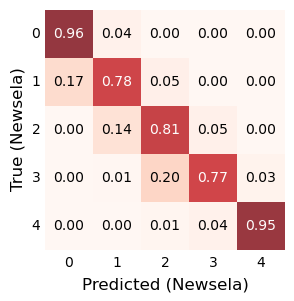
\includegraphics[width=7cm]{pictures/train_newsela_test_newsela.png}
\caption{Confusion matrix of predicted complexity levels after fine-tuning BERT on Newsela vs. true complexity levels.}
\label{table:comp_pred}
\end{figure}

The fine-tuned BERT model has an overall {\bf accuracy of 0.764} on individual text segments, and a document-level {\bf accuracy of 0.844} in our held-out test set. We also report the accuracy of our complexity prediction model for each complexity level in the confusion matrix in Figure \ref{table:comp_pred}. L0 and L4 documents were almost always correctly classified, while the complexity of L1, L2, and L3 documents was less accurately predicted. However, when the model made a mistake, it was in most cases only one level off. From these results, we can conclude that fine-tuning BERT is a very effective method for predicting in-domain document-level complexity.

\subsection{Cross-Domain Experiment and Results}

While our in-domain results are quite promising, in order for this approach to be practically useful, our model must be able to perform well across different domains. To simulate this setting, we leverage additional datasets. The first the Weebit corpus which consists of a combination of two corpora created for different age groups \citep{vajjala2012improving}: the WeeklyReader corpus \footnote{WeeklyReader has merged with its parent company ScholasticNews, so these articles can now be found at https://scholasticnews.scholastic.com} and the BBC-Bitesize website\footnote{http://www.bbc.co.uk/bitesize}.  The final Weebit corpus consists of the following levels from these corpora: Level 2 (corresponding to grade level 2 and children ages 7-8); Level 3 (grade 3, ages 8-9); and Level 4 (grade 4, ages 9-10); KS3 (ages 11-14) and GCSE (ages 14-16).

%, which comes an educational newspaper that writes articles covering a range of non-fiction topics and directed at four reading levels: Level 2, corresponding to grade level 2, and children ages 7-8; Level 3 (grade 3, ages 8-9); Level 4 (grade 4, ages 9-10) and Senior (grades 5-6, ages 10-12). These levels were determined by leveraging an article's \textit{Lexile}, which is a framework created by MetaMetrics, Inc. The Lexile measure uses quantitative measures based on individual words and the lengths of sentences\footnote{https://lexile.com/parents-students/understanding-your-lexile-measure/the-science-behind-lexile-measures/}.
%While WeeklyReader is a very useful corpus on its own, but is relatively limited in terms of the  range of reading levels. Thus, Weebit also leverages the BBC-Bitesize website, which consists of articles from four \textit{different} grade levels: Key Stage 1, or KS1, corresponding to children ages 5-7; KS2 (ages 8-11); KS3 (ages 11-14); and the level General Certificate of Secondary Education, or GCSE (ages 14-16). Note that it is unclear how the levels on this website were originally created. 

We also introduce a new corpus which consists of 38,639 articles extracted from the Choosito website (henceforth the Choosito corpus) manually labeled at four reading levels: Early (grade levels 2-4); Emerging (grades 5-7); Fluent (grades 8-10); and Advanced (grades 11-12).\footnote{The Choosito corpus was compiled by Jaime Rojas at Choosito, Inc., and was shared with us for this work.)} During corpus creation, any article that contained a sentence with more than 100 words was removed. This was done because we found that these sentences generally consisted of lists of items, which made the text extracted from these articles difficult to parse.

\begin{table*}
\begin{center}
\small
\begin{tabular}{| c c | c c | c c | c c |} \hline
\multirow{2}{1cm}{\textbf{Grade}} & \multirow{2}{1cm}{\textbf{Age}} & \multicolumn{2}{|c|}{\textbf{Newsela}} & \multicolumn{2}{|c|}{\textbf{Weebit}} & \multicolumn{2}{|c|}{\textbf{Choosito}} \\
& & \textbf{Level} & \textbf{\# Articles} & \textbf{Level} & \textbf{\# Articles} & \textbf{Level} & \textbf{\# Articles} \\ \hline
2 & 7-8 & \multirow{11}{1cm}{\centering varies} & 35 & Level 2 & 629 & Early & \multirow{3}{1cm}{\centering 4,044} \\
3 & 8-9 & & 124 & Level 3 & 801 & Early & \\ 
4 & 9-10 & & 1,064 & Level 4 & 814 & Early & \\ 
5 & 10-11& & 864 & KS3 & \multirow{4}{1cm}{\centering 644} & Emerging & \multirow{3}{1cm}{\centering 14,283} \\
6 & 11-12 & & 680 & KS3 & & Emerging & \\
7 & 12-13 & & 685 & KS3 & & Emerging & \\
8 & 13-14 & & 743 & KS3 & & Fluent & \multirow{3}{1cm}{\centering 13,944} \\
9 & 14-15 & & 338 &  GCSE & \multirow{2}{1cm}{\centering 3,500} & Fluent & \\
10 & 15-16 & & 22 & GCSE & & Fluent & \\
11 & 16-17 & & 2 & N/A & N/A & Advanced & \multirow{2}{1cm}{\centering 6,368} \\
12 & 17-18 & & 1,093 & N/A & N/A & Advanced & \\ \hline
\end{tabular}
\end{center}
\caption{\label{tab:reading_levels} Comparison of reading levels across the Newsela, Weebit, and Choosito corpora.}
\end{table*}

These corpora align documents with school grade levels. The Newsela corpus does initially use grade level to ensure that the five aligned documents are written at 5 different complexity levels, but these do not always correspond to the same grade levels. %Note that for this grade level, Newsela also computes an article's \textit{Lexile} score. One obvious concern that comes up here is that when training a model to prediction reading level, we're really just teaching the model to reverse engineer the Lexile measure framework. This is a legitimate criticism, and in this section we do need to rely on the admittedly large assumption that the Lexile framework perfectly captures readability. However, this limitation is one of the main reasons that we attempted transfer on the Choosito corpus, as this relies on manual readability annotations.
The 1,130 aligned documents in the first version of Newsela (Newsela V1) still contain this grade level information. However, this is not the case for Newsela V2, which is the most commonly used version in simplification studies. In order to fairly compare across these corpora, we used Newsela V1 along with its grade level information, and re-organized Newsela levels depending on the corpus used for training/testing. The distribution of documents across grade levels for the Newsela, Weebit, and Choosito corpora is shown in Table \ref{tab:reading_levels}. As we can see, the grade distribution of Newsela articles is relatively inconsistent; there are over 1,000 articles at grade levels 4 and 12, but less than 50 at levels 2, 10, and 11.

\begin{figure}
    \centering
    \begin{subfigure}[c]{.31\textwidth}
    \centering
    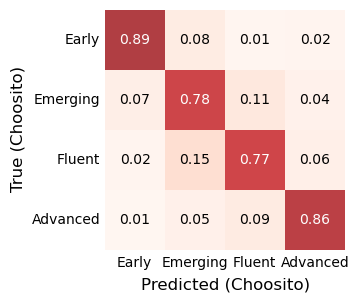
\includegraphics[width=\textwidth]{pictures/train_choosito_test_choosito.png}
    \end{subfigure}%
    \hfill
    \begin{subfigure}[c]{.31\textwidth}
    \centering
    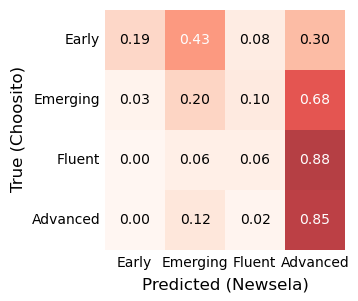
\includegraphics[width=\textwidth]{pictures/train_newsela_test_choosito.png}
    \end{subfigure}%
    \hfill
    \begin{subfigure}[c]{.31\textwidth}
    \centering
    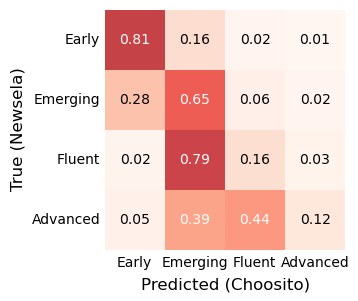
\includegraphics[width=\textwidth]{pictures/train_choosito_test_newsela.png}
    \end{subfigure}
    \newline \newline \newline
    \begin{subfigure}[c]{.31\textwidth}
    \centering
    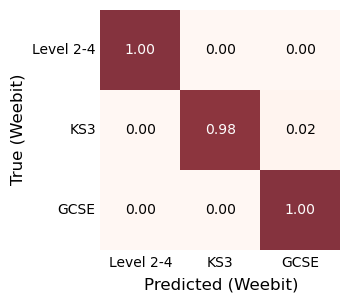
\includegraphics[width=\textwidth]{pictures/train_weebit_test_weebit.png}
    \end{subfigure}%
    \hfill
    \begin{subfigure}[c]{.31\textwidth}
    \centering
    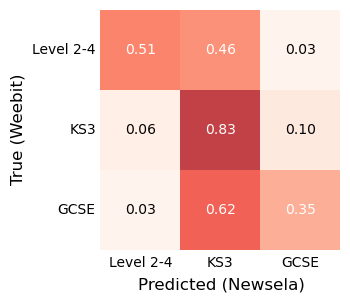
\includegraphics[width=\textwidth]{pictures/train_newsela_test_weebit.png}
    \end{subfigure}%
    \hfill
    \begin{subfigure}[c]{.31\textwidth}
    \centering
    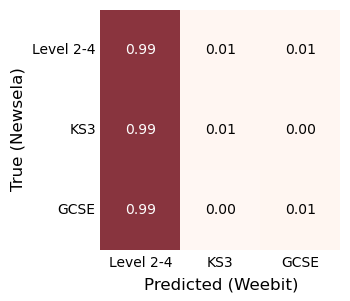
\includegraphics[width=\textwidth]{pictures/train_weebit_test_newsela.png}
    \end{subfigure}
    \caption{Confusion matrix for in-domain and out-of-domain performance across reading levels. The first row shows the performance of training/testing on the Choosito corpus, training on Newsela/testing on Choosito, and finally training on Choosito/testing on Newsela. The second row shows the performance of training/testing on the Weebit corpus, training on Newsela/testing on Weebit, and finally training on Weebit/testing on Newsela. Note that when using Newsela, we modify the reading levels to match the second corpus.}
    \label{fig:domain_reading_levels}
\end{figure}

%To align with Weebit, we first merge Weebit Levels 2-4 together. From there, from each set of 5 aligned Newsela articles, we identify any articles written at grade levels 2-4, articles written at grades 5-8, and articles written at grades 9-10. If there are multiple articles found within one level, we simply select one at random; this is to avoid confusing the model by passing it two of the same articles written at different complexity levels. This process results in 1,104 Newsela articles at Levels 2-4, 1,130 at KS3, and 353 at GCSE. Due to the discrepancy in class sizes, we balance the data before training. We do the same process for aligning Newsela to Choosito reading levels, resulting in 985 articles for each of the four levels.

With these corpora, we run six additional complexity prediction experiments: train and test on Choosito articles (in-domain), train on Newsela and test on Choosito (cross-domain); train on Choosito and test on Newsela (cross-domain); train and test on Weebit articles (in-domain); train on Newsela and test on Weebit (cross-domain); and train on Weebit and test on Newsela (cross-domain). The resulting confusion matrices are shown in Figure \ref{fig:domain_reading_levels}. As we can see, our models were again able to achieve consistently high performance in the in-domain experiments, but in the cross-domain settings the performance sharply decreases. A qualitative exploration of the data reveals that Weebit and Choosito are composed of noisier web articles which often contain more incomplete sentences and pictures captions. Hence, it seems that a significant change in text style has a significant impact on a model's ability to predict complexity. This is an important limitation to consider if our goal is to develop a generally-applicable complexity prediction model.

\section{Re-ranking Retrieved Documents by Complexity} \label{sec:rerank_ir}

We use our in-domain complexity prediction model trained on Newsela (Section \ref{sec:comp_pred}) to re-rank the documents in our initial retrieval experiments (Section \ref{sec:retrieval}). Our goal is to boost the documents that are predicted to be at the desired level in the ranking. In this experiment, we rank articles using the KAAD (Keep All Aligned Documents) configuration, which makes the task of finding the aligned document at the correct level more difficult.

During re-ranking, we first boost the rank of documents at the desired level (e.g., L0), followed by documents at the next closest level (L1), etc. We apply this re-ranking mechanism to both of our retrieval experiments, i.e. using only Newsela documents and augmenting the corpus with NYT articles.

\subsection{Results}

The results obtained after applying the re-ranking mechanism to the retrieval experiment restricted to Newsela articles are shown in Table \ref{table:ir_rerank_newsela}. The results obtained in the setting where NYT articles are included are shown in Table \ref{table:ir_rerank_nyt}. Prior to re-ranking, the L3 article is almost always ranked highest by both BERT and SBERT; this makes sense, as aligned documents at levels L3 and L4 generally are most similar. Interestingly, in Table \ref{table:ir_rerank_newsela}, we see that SBERT ranks the L2 document as most similar to its corresponding L4 document 18\% of the time (Top-1 Accuracy), while BERT does so a negligible 0.6\% of the time. This again supports our previous finding that SBERT better captures semantic similarity across complexity levels.

\begin{table*}
\begin{center}
\scriptsize
\begin{tabular}{|cc|cc|cc|cc|cc|}
\hline
\multirow{3}{1.7cm}{\centering \textbf{Embedding Method}} & \multirow{3}{1.2cm}{\centering \textbf{Re-Ranked}} &  \multicolumn{8}{|c|}{\textbf{Target Aligned Document CL (Newsela only)}} \\
& & \multicolumn{2}{|c|}{\textbf{L3}} & \multicolumn{2}{|c|}{\textbf{L2}} & \multicolumn{2}{|c|}{\textbf{L1}} & \multicolumn{2}{|c|}{\textbf{L0}} \\
& & MRR & Top1Acc & MRR & Top1Acc & MRR & Top1Acc & MRR & Top1Acc \\ \hline
\multirow{2}{1.7cm}{\centering BERT} & No & \textbf{0.995} & \textbf{0.993} & 0.502 & 0.006 & 0.287 & 0 & 0.121 & 0 \\
& Yes & 0.784 & 0.782 & \textbf{0.714} & 0.645 & \textbf{0.691} & 0.639 & 0.616 & 0.521 \\ \hline
\multirow{2}{1.7cm}{\centering SBERT} & No & 0.859 & 0.753 & 0.543 & 0.182 & 0.353 & 0.041 & 0.235 & 0.016 \\
& Yes & 0.776 & 0.767 & \textbf{0.714} & 0.654 & \textbf{0.693} & \textbf{0.644} & \textbf{0.731} & \textbf{0.629} \\ \hline
\end{tabular}
\end{center}
\caption{\label{table:ir_rerank_newsela} Ranking results for retrieving aligned Newsela documents at four complexity levels (CL), using the KAAD approach. For each embedding method, we report results with and without re-ranking.}
\end{table*}

\begin{table*}
\begin{center}
\scriptsize
\begin{tabular}{|cc|cc|cc|cc|cc|}
\hline
\multirow{3}{1.7cm}{\centering \textbf{Embedding Method}} & \multirow{3}{1.2cm}{\centering \textbf{Re-Ranked}} &  \multicolumn{8}{|c|}{\textbf{Target Aligned Document CL (Newsela + NYT Distractors)}} \\
& & \multicolumn{2}{|c|}{\textbf{L3}} & \multicolumn{2}{|c|}{\textbf{L2}} & \multicolumn{2}{|c|}{\textbf{L1}} & \multicolumn{2}{|c|}{\textbf{L0}} \\
& & MRR & Top1Acc & MRR & Top1Acc & MRR & Top1Acc & MRR & Top1Acc \\ \hline
\multirow{2}{1.7cm}{\centering BERT} & No & \textbf{0.993} & \textbf{0.989} & 0.488 & 0.006 & 0.203 & 0 & 0.054 & 0 \\
& Yes & 0.784 & 0.782 & \textbf{0.713} & \textbf{0.645} & \textbf{0.688} & \textbf{0.634} & 0.599 & 0.512 \\ \hline
\multirow{2}{1.7cm}{\centering SBERT} & No & 0.814 & 0.711 & 0.480 & 0.168 & 0.262 & 0.035 & 0.136 & 0.011 \\
& Yes & 0.770 & 0.760 & 0.701 & 0.638 & 0.675 & 0.622 & \textbf{0.691} & \textbf{0.593} \\ \hline
\end{tabular}
\end{center}
\caption{\label{table:ir_rerank_nyt} Ranking results for retrieving aligned Newsela documents at four complexity levels (CL), including the additional NYT distractor articles. We again use the KAAD approach, and report results with and without re-ranking.}
\end{table*}

We see that re-ranking significantly increases performance when retrieving L2, L1, and L0 documents. After incorporating re-ranking, SBERT no longer outperforms BERT for L2 and L1 documents, though it is still more effectively in identifying L0 documents. This demonstrates that a two-step process of embedding-based retrieval and re-ranking based on predicted complexity, can be effectively used to retrieve documents at any complexity level. On the other hand, re-ranking does not help when retrieving L3 articles. This is because when an article's complexity level is incorrectly predicted, relying on that prediction for re-ranking will lead to that article being pushed down in the list. However, since embedding-based methods are already quite effective at retrieving related documents at similar complexity levels, re-ranking is unnecessary in this case.

\section{Summary}

In this chapter, we present a reformulation of text simplification as a retrieval task. Our overall goal is to take in a document $D$ and, after identifying concepts that are critical for understanding $D$, retrieve a document related to each concept that is more appropriate for a user. To this end, the first section of this chapter focuses on critical concept identification. We describe in detail various statistical approaches commonly used for the related task of keyphrase extraction, and propose several BERT-based approaches that utilize embedding similarity to rank concepts. We also present two baseline approaches that leverage Wikipedia categories. To test these methods, we create a high-quality concept identification evaluation corpus using trained annotators. We surprisingly find that both the statistical and Wikipedia-based baselines outperform our BERT-based approaches. This is likely because comparing a concept embedding is difficult to compare to a title or document embedding, which both contain many non-concepts.

In the second part of this chapter, we focus on the task of retrieving related documents at varying complexity levels. We show that embeddings generated from contextualized language models are able to effectively rank highly aligned documents from similar complexity levels, this is not the case when aligned documents are of more disparate complexities. To circumvent this issue, we propose a secondary ranking mechanism that predicts each document's complexity, and then leverages this prediction to re-rank the documents. With this, we are able to effectively retrieve related documents at any desired complexity level. This holds true even in a more challenging setting, where we have over one million distractor documents. While these results are indeed promising, we also discuss the fact that complexity can be domain-specific. We present cross-domain experiments which show the difficulty of fine-tuned complexity prediction models to maintain performance when transferring to a new domain.

\biblio
\end{document}
